\documentclass{article}

\usepackage{hyperref}
\usepackage{amsmath}
\usepackage{graphicx}
%\usepackage{subcaption}
\usepackage{epstopdf}
\usepackage{color}

\usepackage{times}
\usepackage{bm}

% Page layout
\hoffset -0in
\voffset -1in
\oddsidemargin 0in
\textheight 9.3in
\textwidth 6.3in

\setlength{\parindent}{0pt}

\graphicspath{{figures/}}

\begin{document}
\section*{COMPUTATIONAL METHODS IN MECHANICS: Assignment 9}
Vesa-Ville Hurskainen, 20 Apr 2018\\
\href{https://github.com/VesaVilleHurskainen/cmim2018}{GitHub repository}


\section*{Introduction}
This is a report for the ninth and final assignment of the course \textit{Computational Methods in Mechanics}, concerning optimization. The assignment consists of four tasks, which are as follows:
\begin{enumerate}
	\setlength\itemsep{0pt}
	\item To expand the previously-made general purpose program with translational joints and point forces.
	\item To model a robot gripper and repeat the optimization procedure described in the material.
	\item To test different optimization procedure settings.
	\item To try to use \texttt{fminsearch} with penalty method for the optimization.
\end{enumerate}

\section*{Methods}
First, the translational joints were implemented to the previously written program, in addition to elementary 1 DOF locking joints for fixing rotation between bodies 2a and 2b. Then, point forces (direction defined in global coordinate frame) were implemented. Finally, the described optimization procedure was performed.\\

Since the gripper is symmetric and the trajectories of the two "fingers" are therefore identical (mirrored), the optimization can be performed using a half-system model. The optimization is done using the script \texttt{optimizeGrabber}, for which the half-system model is defined in function \texttt{optFun}. The whole system can then be simulated with optimized geometry and the results visualized using the script \texttt{inputData\_grabber}.

\section*{Results}
The dynamic simulations were performed using the following parameters: $t = 0 \dots 1$ s, $\Delta t = 0.01$ s, $\rho_L = 2$ kg/cm, $F = [-400~~0]^\text{T}$ N. Baumgarte stabilization was used for the constraints, with the parameters $\alpha = \beta = 100$. The MATLAB solver \texttt{ode45} was employed, and gravity was not taken into account. For optimization, point coordinates according to the original geometry were used as starting values.\\

Diagrams of the original and optimized (using interior-point algorithm) geometries are presented in Figure~\ref*{fig:geometry}. The resulting point coordinates and optimization statistics when using different optimization algorithms are presented in Table~\ref*{tab:results}.

\begin{figure}[htb]
	\centering
	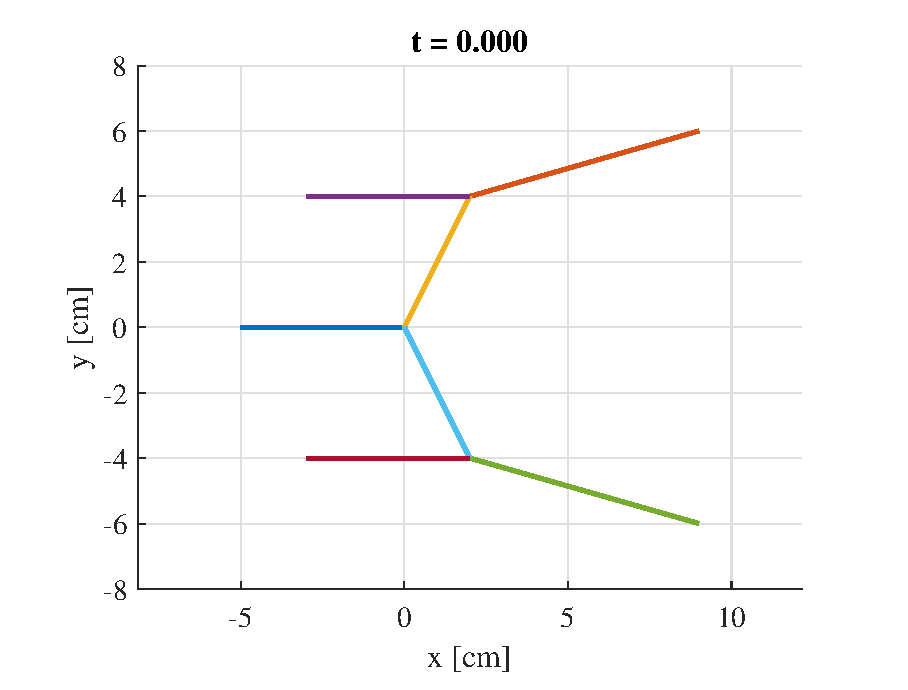
\includegraphics[width=0.45\textwidth]{unoptimized.eps}~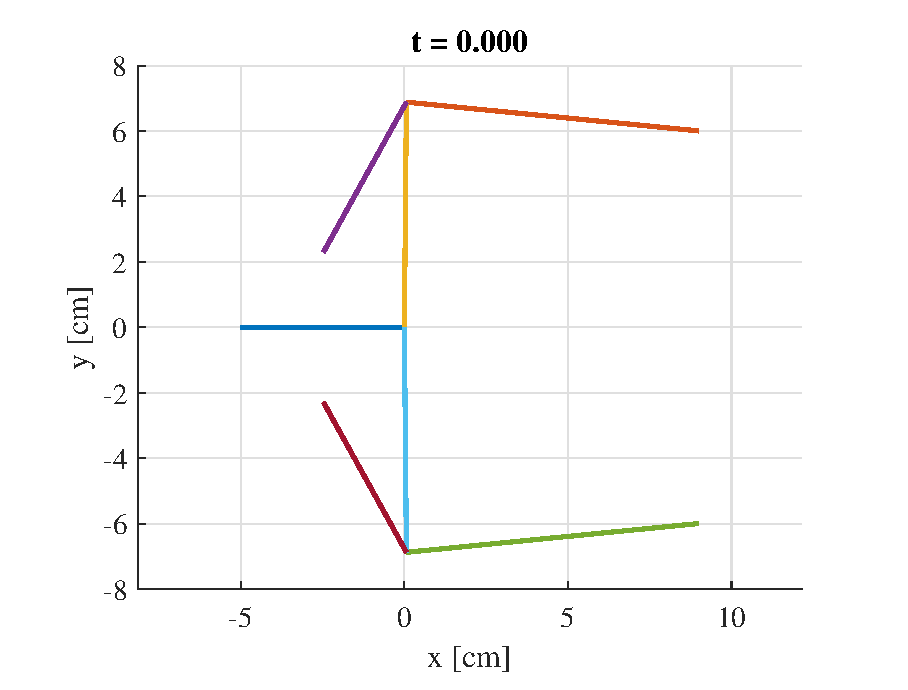
\includegraphics[width=0.45\textwidth]{optimized.eps}
	\caption{Initial versus optimized gripper geometry at $t = 0$, interior-point algorithm.\label{fig:geometry}}
\end{figure}

\begin{table}[htb]
	\centering
	\caption{Results and optimization statistics for different algorithms.\label{tab:results}}
	\begin{tabular}{|l|c|c|c|}
		\hline
		Algorithm & Result & Iterations & Evaluations\\
		\hline
		interior-point & $B = \begin{bmatrix} 0.0687 \\ 6.6047 \end{bmatrix} C = \begin{bmatrix} -3.0713 \\ 1.2103 \end{bmatrix}$ & 53 & 437\\
		sqp            & $B = \begin{bmatrix} 0.0544 \\ 6.5556 \end{bmatrix} C = \begin{bmatrix} -3.1686 \\ 1.0000 \end{bmatrix}$ & 69 & 480\\
		active-set     & $B = \begin{bmatrix} 0.1229 \\ 7.0000 \end{bmatrix} C = \begin{bmatrix} -2.5400 \\ 2.1516 \end{bmatrix}$ & 30 & 189\\
		\hline
	\end{tabular}
\end{table}

\section*{Analysis}
As we can see from Table~\ref*{tab:results}, there are some differences in the results produced by the different optimization algorithms. Notably, several results are close to the defined optimization limits (e.g. y-coordinate of point B). This means that modifying the limits could provide drastically different results.

\end{document}